\chapter{序論}
我々の身の回りにある物質を構成する最小単位は素粒子である。
物質の最小単位である素粒子と、素粒子の相互作用を記述した理論として標準模型が存在している。素粒子物理学において、自然界には電磁相互作用、強い相互作用、弱い相互作用、重力相互作用といった4種類の基本相互作用が存在すると考えられており、標準模型では重力相互作用以外の3種類の相互作用が記述されている。
標準模型は図\ref{fig:標準模型}に示すように、12種類のフェルミオン、4種類のゲージボソン、ヒッグス粒子の計17種類の粒子から構成されており、2012年に唯一実験的に未確認であったヒッグス粒子が発見された\cite{article:Higgs_boson}。
\begin{figure}[tb]
  \centering
  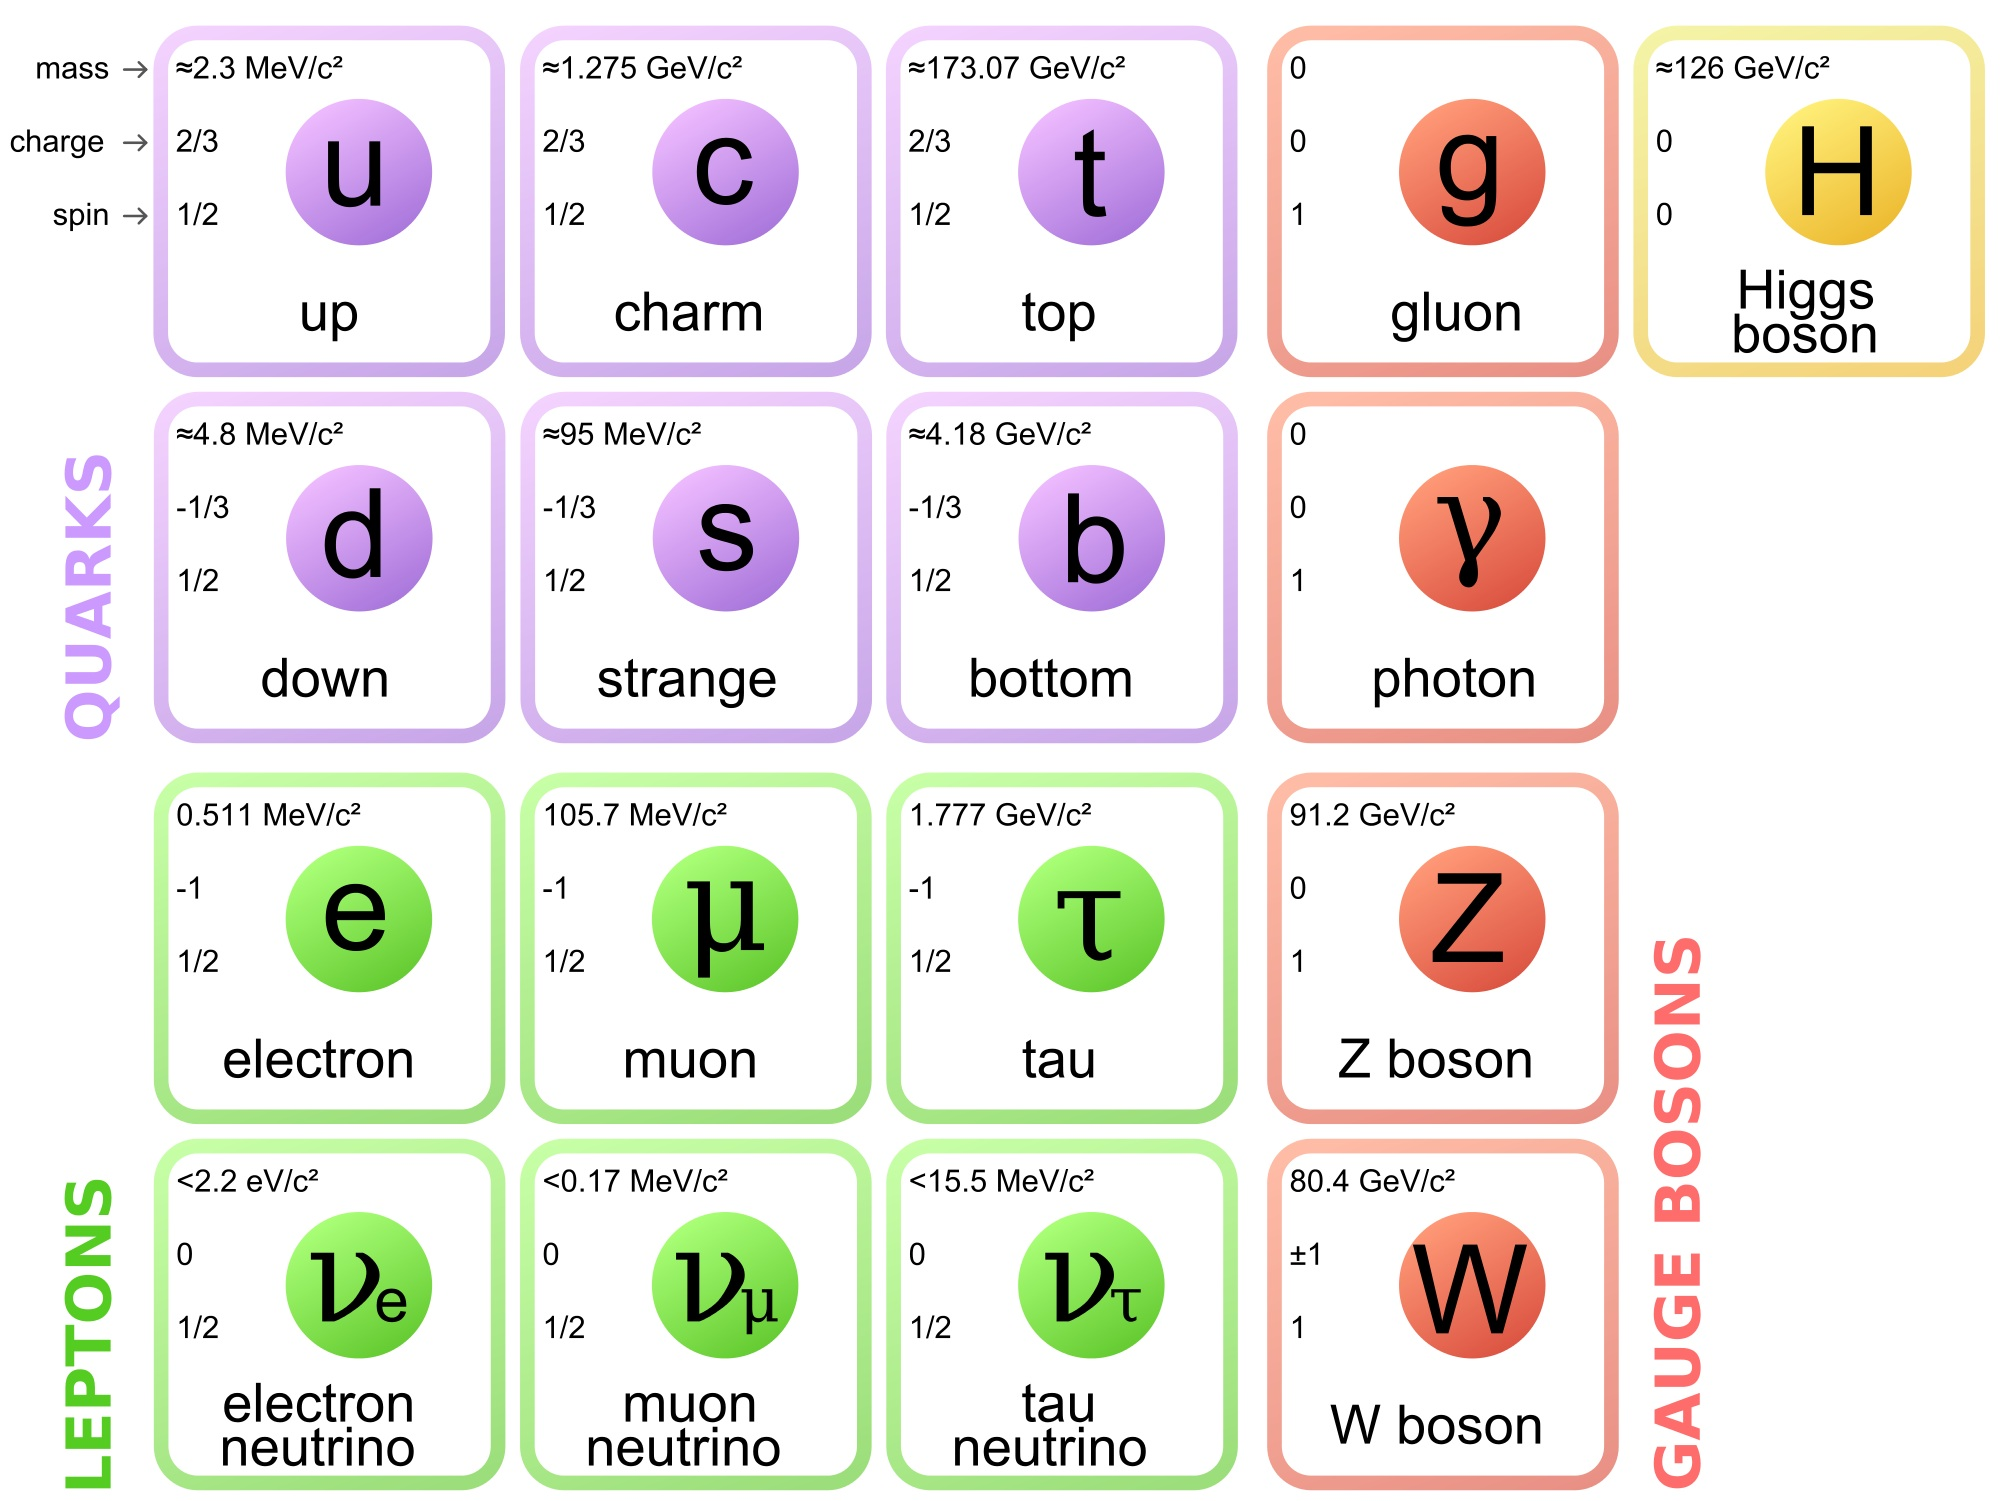
\includegraphics[clip, width=10cm]{fig/1/standardmodel.jpg}
  \caption{標準模型を構成する17種類の素粒子\cite{article:elementary_particles}。}
  \label{fig:標準模型}
\end{figure}

現在、標準模型は多くの物理事象を説明することができているが、暗黒物質の存在やヒッグス粒子の質量階層性問題などの多くの未解決問題が残されている。
この問題を解決するためには、標準模型を超える新しい物理が必要であり、この新物理を探索するためのアプローチとして世界中で様々な実験が行われている。

新物理探索の実験の一つとして、ジュネーブ郊外に位置する欧州原子核研究機構~(CERN)~\cite{article:CERN}の地下に設置された Large Hadron Collider~(LHC)~\cite{article:LHC}を用いる高エネルギーの陽子陽子衝突実験がある。このLHCを使った衝突実験の1つであるATLAS実験では、ATLAS検出器と呼ばれる大型汎用検出器を用いて陽子-陽子衝突によって生成される粒子を検出し、TeVスケールの物理事象までの測定を行い標準理論を構成する素粒子の精密測定や超対称性粒子の探索を目的としている~\cite{article:ATLAS}。

LHC における陽子-陽子衝突の頻度は40~MHzであるが、計算機リソースやデータ記憶容量など制限から全ての衝突事象を保存することができない。そのため、トリガーシステムを使った事象選別を行うことで膨大な量の衝突事象から物理として興味のある事象を選別し、取得可能なデータ量まで事象数を減らして保存している。
ATLAS検出器では大きく分けて2段階のトリガーシステムを実装している。1段目にはハードウェアベースの高速処理が可能な初段トリガー(Level-1 Trigger:L1 Trigger)があり、全事象に対しトリガー判定を行うことで100~kHz以下まで事象数を落とす。2段目にはソフトウェアベースで精密処理が可能な後段トリガー(High-Level Trigger:HLT)があり、L1 Triggerで選別した事象をさらに数kHzまで落とす。

本研究では、この初段トリガー、特にミューオンの運動量を指針として事象選別を行うエンドキャプ部の初段ミューオントリガーに着目する。
ATLAS検出器の最外層に位置するミューオン検出器には衝突点からのミューオンのみが飛来するため、粒子の同定が容易であるため短時間でトリガーを発行することができる。さらに、ヒッグス粒子の崩壊先であるZボソンやWボソンの終状態として高い運動量のミューオンが観測されやすいことや、ボトムクォークやチャームクォークが含まれる粒子の終状態には運動量が低いミューオンが含まれる。そのため、ミューオンは陽子-陽子衝突実験において様々な物理事象のサインとして重宝されている。

LHC及びATLAS検出器は2018年から2021年までの期間にアップグレードが行われ、2022年からRun-3として運転が再開された。Run-3では陽子-陽子衝突の重心系エネルギーの増強や高いルミノシティでの安定した運転に伴い事象頻度がさらに増加する。したがって、限られたデータ容量の中で物理事象を最大効率で取得するために、初段トリガーにおいてもトリガーシステムの改良を行い、トリガー効率を向上させる必要がある。本論文では、ミューオンをターゲットにして事象選別を行う初段エンドキャプ部ミューオントリガーを改良し、トリガー性能の評価について述べる。

本論文は、第\ref{chapter2}章でLHC-ATLAS実験のの概要について述べ、第\ref{chapter3}章で初段ミューオントリガーシステムについて述べる。
第\ref{chapter4}章で機械学習を用いたCWの作成手法の詳細について説明し、第\ref{chapter5}章で作成したCWを用いた際のトリガー性能の評価について述べた後、第\ref{chapter6}章で本研究で開発した作成手法とその成果をまとめ、今後の展望について述べる。


